\documentclass{article}
\usepackage[utf8]{inputenc}
\usepackage[margin=1in]{geometry}
\usepackage{float}
\usepackage{amsmath}
\usepackage{graphicx}
\usepackage{longtable}
\setlength{\parindent}{20pt}
\title{Misura della caratteristica I-V di un transistor BJT}
\author{Matteo Bonazzi, Massimo D'Alessandro Schmidt}


\begin{document}

\maketitle
\begin{abstract}
    Misura della caratteristica I-V di un transistor BJT in configurazione emettitore comune, in due valori differenti della corrente di base \\
    Dal fit lineare dei dati nella regione attiva, si ottengono i parametri $V_{Early}=$ e $R=$.
\end{abstract}

\section{Introduzione}
Per la misura è stato utilizato un transistor BJT di tipo pnp,.......; il transistor è in configurazione a base comune, con base
e collettore collegati a due potenziometri e l'emettitore collegato a terra.\\
Il circuito è realizzato con due potenziometri regolabili, uno regolante la corrente di base $I_b$ con una resitenza di $100k\Omega$, e uno regolante
la corrente di collettore $I_c$, con resitenza pari a $1k\Omega$;

\section{Dati}
Nella configurazione con $I_b=-200\mu A$, si misurano i seguenti valori per $V_{ce}$ e $I_c$:
\begin{longtable}[c]{|l|l|l|l|l|l|l|l|l|}
    \cline{1-4} \cline{6-9}
    $V_{ce}$ (mV) & \begin{tabular}[c]{@{}c@{}}Errore V \\ (mV)\end{tabular} & \begin{tabular}[c]{@{}c@{}}Risoluzione \\ (mV)\end{tabular} & \begin{tabular}[c]{@{}c@{}}Fondo scala \\ (mV/div)\end{tabular} &  & $I_c$ (mA) & \begin{tabular}[c]{@{}c@{}}errore $I_c$  \\ (mA)\end{tabular} & \begin{tabular}[c]{@{}c@{}}Risoluzione \\ (mA)\end{tabular} & \begin{tabular}[c]{@{}c@{}}Fondo scala \\ (mA)\end{tabular} \\ \cline{1-4} \cline{6-9}
    \endfirsthead
    \endhead
    4000          & 160                       & 200                       & 1000                      &  & 36.9       & 0.18                      & 0.1                       & 200                       \\ \cline{1-4} \cline{6-9}
    3800          & 150                       & 200                       & 1000                      &  & 36.5       & 0.18                      & 0.1                       & 200                       \\ \cline{1-4} \cline{6-9}
    3600          & 150                       & 200                       & 1000                      &  & 36         & 0.18                      & 0.1                       & 200                       \\ \cline{1-4} \cline{6-9}
    3400          & 143                       & 200                       & 1000                      &  & 35.6       & 0.18                      & 0.1                       & 200                       \\ \cline{1-4} \cline{6-9}
    3200          & 139                       & 200                       & 1000                      &  & 35.1       & 0.18                      & 0.1                       & 200                       \\ \cline{1-4} \cline{6-9}
    3000          & 135                       & 200                       & 1000                      &  & 34.7       & 0.17                      & 0.1                       & 200                       \\ \cline{1-4} \cline{6-9}
    2900          & 100                       & 200                       & 500                       &  & 34.6       & 0.17                      & 0.1                       & 200                       \\ \cline{1-4} \cline{6-9}
    2700          & 95                        & 200                       & 500                       &  & 34.2       & 0.17                      & 0.1                       & 200                       \\ \cline{1-4} \cline{6-9}
    2500          & 90                        & 100                       & 500                       &  & 33.6       & 0.17                      & 0.1                       & 200                       \\ \cline{1-4} \cline{6-9}
    2400          & 88                        & 100                       & 500                       &  & 33.6       & 0.17                      & 0.1                       & 200                       \\ \cline{1-4} \cline{6-9}
    2200          & 83                        & 100                       & 500                       &  & 33.1       & 0.17                      & 0.1                       & 200                       \\ \cline{1-4} \cline{6-9}
    2000          & 78                        & 100                       & 500                       &  & 32.5       & 0.16                      & 0.1                       & 200                       \\ \cline{1-4} \cline{6-9}
    1900          & 76                        & 100                       & 500                       &  & 32.5       & 0.16                      & 0.1                       & 200                       \\ \cline{1-4} \cline{6-9}
    1700          & 71                        & 100                       & 500                       &  & 32         & 0.16                      & 0.1                       & 200                       \\ \cline{1-4} \cline{6-9}
    1500          & 67                        & 100                       & 500                       &  & 31.4       & 0.16                      & 0.1                       & 200                       \\ \cline{1-4} \cline{6-9}
    1400          & 65                        & 100                       & 500                       &  & 31.2       & 0.16                      & 0.1                       & 200                       \\ \cline{1-4} \cline{6-9}
    1200          & 41                        & 40                        & 200                       &  & 30.8       & 0.15                      & 0.1                       & 200                       \\ \cline{1-4} \cline{6-9}
    1120          & 39                        & 40                        & 200                       &  & 30.6       & 0.15                      & 0.1                       & 200                       \\ \cline{1-4} \cline{6-9}
    1000          & 36                        & 40                        & 200                       &  & 30.2       & 0.15                      & 0.1                       & 200                       \\ \cline{1-4} \cline{6-9}
    800           & 31                        & 40                        & 200                       &  & 29.8       & 0.15                      & 0.1                       & 200                       \\ \cline{1-4} \cline{6-9}
    720           & 29                        & 40                        & 200                       &  & 28.9       & 0.14                      & 0.1                       & 200                       \\ \cline{1-4} \cline{6-9}
    500           & 18                        & 20                        & 100                       &  & 26.5       & 0.13                      & 0.1                       & 200                       \\ \cline{1-4} \cline{6-9}
    400           & 16                        & 20                        & 100                       &  & 24.4       & 0.12                      & 0.1                       & 200                       \\ \cline{1-4} \cline{6-9}
    300           & 10                        & 10                        & 50                        &  & 22         & 0.11                      & 0.1                       & 200                       \\ \cline{1-4} \cline{6-9}
    200           & 7.8                       & 10                        & 50                        &  & 17.08      & 0.085                     & 0.01                      & 20                        \\ \cline{1-4} \cline{6-9}
    50            & 5.2                       & 10                        & 50                        &  & 4.5        & 0.0225                    & 0.01                      & 20                        \\ \cline{1-4} \cline{6-9}
    \caption{\label{tab:Tabella1}{Valori di $V_{ce}$ e $I_c$, per $I_b=200\mu A$}}                                                                                                                        \\
\end{longtable}

Nella configurazione con $I_b=-100\mu A$, si misurano i seguenti valori per $V_{ce}$ e $I_c$:
\begin{longtable}[c]{|l|l|l|l|l|l|l|l|l|} 
    \cline{1-4} \cline{6-9}
    $V_{ce}$ (mV) & \begin{tabular}[c]{@{}c@{}}Errore V \\ (mV)\end{tabular} & \begin{tabular}[c]{@{}c@{}}Risoluzione \\ (mV)\end{tabular} & \begin{tabular}[c]{@{}c@{}}Fondo scala \\ (mV/div)\end{tabular} &  & $I_c$ (mA) & \begin{tabular}[c]{@{}c@{}}errore $I_c$  \\ (mA)\end{tabular} & \begin{tabular}[c]{@{}c@{}}Risoluzione \\ (mA)\end{tabular} & \begin{tabular}[c]{@{}c@{}}Fondo scala \\ (mA)\end{tabular} \\ \cline{1-4} \cline{6-9}
    \endfirsthead
    \endhead
    4000          & 156                       & 200                       & 1000                       &  & 21.7       & 0.11                       & 0.1                        & 200                        \\ \cline{1-4} \cline{6-9}
    3800          & 152                       & 200                       & 1000                       &  & 21.6       & 0.11                       & 0.1                        & 200                        \\ \cline{1-4} \cline{6-9}
    3600          & 147                       & 200                       & 1000                       &  & 21.3       & 0.11                       & 0.1                        & 200                        \\ \cline{1-4} \cline{6-9}
    3400          & 143                       & 200                       & 1000                       &  & 21.1       & 0.11                       & 0.1                        & 200                        \\ \cline{1-4} \cline{6-9}
    3200          & 108                       & 200                       & 1000                       &  & 21         & 0.11                       & 0.1                        & 200                        \\ \cline{1-4} \cline{6-9}
    3000          & 135                       & 200                       & 1000                       &  & 21         & 0.11                       & 0.1                        & 200                        \\ \cline{1-4} \cline{6-9}
    2900          & 100                       & 100                       & 500                        &  & 20.7       & 0.10                       & 0.1                        & 200                        \\ \cline{1-4} \cline{6-9}
    2700          & 95                        & 100                       & 500                        &  & 20.4       & 0.10                       & 0.1                        & 200                        \\ \cline{1-4} \cline{6-9}
    2500          & 90                        & 100                       & 500                        &  & 20.4       & 0.10                       & 0.1                        & 200                        \\ \cline{1-4} \cline{6-9}
    2400          & 87                        & 100                       & 500                        &  & 20.2       & 0.10                       & 0.1                        & 200                        \\ \cline{1-4} \cline{6-9}
    2200          & 83                        & 100                       & 500                        &  & 19.96      & 0.10                       & 0.01                       & 20                         \\ \cline{1-4} \cline{6-9}
    2000          & 78                        & 100                       & 500                        &  & 19.84      & 0.099                      & 0.01                       & 20                         \\ \cline{1-4} \cline{6-9}
    1900          & 76                        & 100                       & 500                        &  & 19.72      & 0.099                      & 0.01                       & 20                         \\ \cline{1-4} \cline{6-9}
    1700          & 71                        & 100                       & 500                        &  & 19.49      & 0.097                      & 0.01                       & 20                         \\ \cline{1-4} \cline{6-9}
    1500          & 67                        & 100                       & 500                        &  & 19.26      & 0.096                      & 0.01                       & 20                         \\ \cline{1-4} \cline{6-9}
    1400          & 65                        & 100                       & 500                        &  & 19.14      & 0.096                      & 0.01                       & 20                         \\ \cline{1-4} \cline{6-9}
    1200          & 41                        & 50                        & 200                        &  & 18.81      & 0.094                      & 0.01                       & 20                         \\ \cline{1-4} \cline{6-9}
    1080          & 38                        & 50                        & 200                        &  & 18.69      & 0.093                      & 0.01                       & 20                         \\ \cline{1-4} \cline{6-9}
    1000          & 36                        & 50                        & 200                        &  & 18.58      & 0.093                      & 0.01                       & 20                         \\ \cline{1-4} \cline{6-9}
    800           & 31                        & 50                        & 200                        &  & 18.42      & 0.092                      & 0.01                       & 20                         \\ \cline{1-4} \cline{6-9}
    720           & 29                        & 50                        & 200                        &  & 18.29      & 0.091                      & 0.01                       & 20                         \\ \cline{1-4} \cline{6-9}
    500           & 18                        & 20                        & 100                        &  & 17.74      & 0.089                      & 0.01                       & 20                         \\ \cline{1-4} \cline{6-9}
    400           & 15                        & 20                        & 100                        &  & 17.11      & 0.086                      & 0.01                       & 20                         \\ \cline{1-4} \cline{6-9}
    300           & 10                        & 10                        & 50                         &  & 15.78      & 0.079                      & 0.01                       & 20                         \\ \cline{1-4} \cline{6-9}
    200           & 8                         & 10                        & 50                         &  & 12.46      & 0.062                      & 0.01                       & 20                         \\ \cline{1-4} \cline{6-9}
    50            & 5                         & 10                        & 50                         &  & 3.19       & 0.016                      & 0.01                       & 20                         \\ \cline{1-4} \cline{6-9}
    
    \caption{\label{tab:Tabella2}{Valori di $V_{ce}$ e $I_c$, per $I_b=100\mu A$}}                                                                                                                            \\
\end{longtable}


\section{Analisi dati}
\begin{figure}[H]
    \centering
    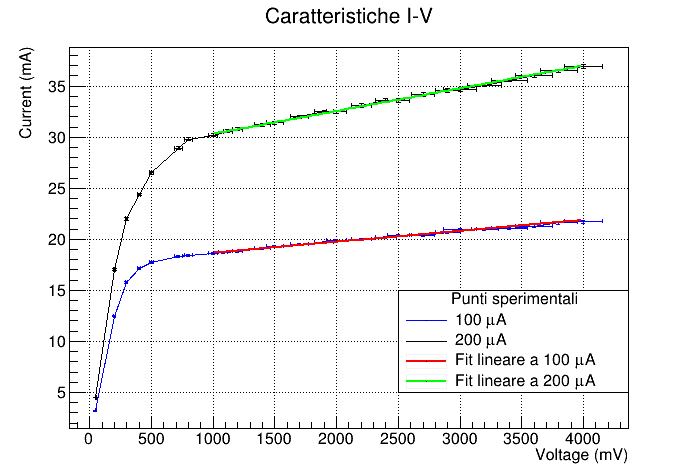
\includegraphics[width=0.8\textwidth]{Multigraph.png}
    \caption{\label{fig:multigraph}Grafico delle caratterste I-V del transistor, nelle due configurazioni delle correnti di base $I_b$}
\end{figure}
Per $V_{ce}$ nel range $1-4 V$, cioè nella regione attiva del transistor, si opera un fit lineare del tipo:
\begin{equation}
    V_{ce} = a + b I_c\\
\end{equation}
Dove a rappresenta la tensione di Early $V_{Ea}$, e b rappresenta la resistenza del circuito; dal fit si ottengono i seguenti valori:
\begin{equation}
    \begin{aligned}
        V_{Ea,100\mu A}=(16\pm 6) V \\
        R_{100\mu A}=(931 \pm 30) \Omega \\
        V_{Ea,200\mu A}=(13\pm 4) V \\
        R_{200\mu A}=(449 \pm 13) \Omega\\
    \end{aligned}
\end{equation} 
Dalle stime fornite dal fit è possibile ricavare i valori delle conduttanze, che risultano essere:
\begin{equation}
    \begin{aligned}
        g_{100 \mu A}=(1.07 \pm 0.04) m\Omega^{-1} \\
        g_{200 \mu A}=(2.22 \pm 0.07) m\Omega^{-1}\\
    \end{aligned}
\end{equation}




\end{document}